
\section{Marco Teórico}

\subsection{Amplificadores Realimentados por Tensión (VFA)}

El Amplificador Operacional clásico, o Amplificador Realimentado por Tensión (VFA, por sus siglas en inglés), es un dispositivo fundamental en la electrónica analógica.

\subsubsection{Características Principales}
\begin{figure}[H]
    \centering
    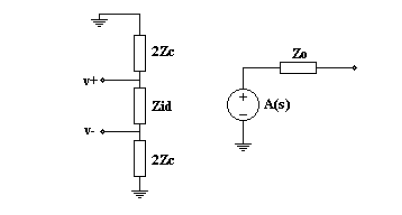
\includegraphics[width=0.5\linewidth,height=0.32\textheight,keepaspectratio]{Imagenes/modelo_VFA.png}
    \caption{Modelo real del VFA}
    \label{fig:modelo_VFA}
\end{figure}

El modelo en pequeña señal de un VFA, \autoref{fig:modelo_VFA}, se caracteriza por poseer una impedancia de entrada en modo diferencial ($Z_{id}$), típicamente con componentes resistivas superiores al megaohm y capacitivas de unos pocos picofaradios, y una impedancia de modo común ($Z_C$) la cual suele ser de 1 o 2 ordenes mayor a la anterior. Por otro lado, su impedancia de salida ($Z_o$) es muy baja, del orden de las decenas de ohms. El dispositivo presenta una ganancia de tensión a lazo abierto en modo diferencial ($A_d$) muy elevada (típicamente en torno a los $100\text{ dB}$) y una ganancia en modo común ($A_c$) prácticamente nula. Quedando su salida definida por 

\begin{equation}
    V_o = A_d(s) \cdot (V^+- V^-)+ A_c(s) \cdot (\dfrac{V^+ + V^-}{2})
    \label{eq:ecuacion_general_1}
\end{equation}
Siendo:
\begin{align}
    \text{Tensión de modo diferencial:}&\ V_d = V^+- V^-\\
    \text{Tensión de modo común:}&\ V_c = \dfrac{V^+ + V^-}{2}\\
    \text{Relación de rechazo de modo común}&\ RRMC = \dfrac{A_d(s)}{A_c(s)}
\end{align}

En la \autoref{fig:modelos_VFA_2} se tienen dos modelos, un modelo simplificado y un modelo idealizado.
El modelo simplificado contempla una impedancia de entrada resistiva ($R_i$) mientras que en el modelo idealizado se asume un cortocircuito virtual entre los terminales de entrada ($V^+ = V^-$). Esto se debe que en el modelo idealizado se consideran: $ A_{d}(s) \xrightarrow[]{}{\infty}$,  $A_c(s) \xrightarrow[]{}0$ y una $RRMC\ \xrightarrow[]{}{\infty}$. Por lo tanto, para que la \autoref{eq:ecuacion_general_1} tenga un valor finito se debe cumplir la \autoref{eq:condicion_ideal}.
\begin{equation}
    V^+ = V^-
    \label{eq:condicion_ideal}
\end{equation}

\begin{figure}[H]
  \centering
  \begin{subfigure}{0.45\linewidth}
    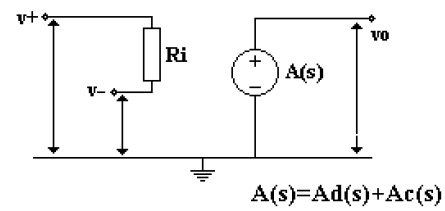
\includegraphics[width=\linewidth,height=0.32\textheight,keepaspectratio]{Imagenes/modelo_simplificado_VFA.png}
    \caption{Modelo simplificado}
  \end{subfigure}
  \begin{subfigure}{0.45\linewidth}      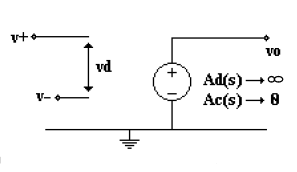
\includegraphics[width=\linewidth,height=0.32\textheight,keepaspectratio]{Imagenes/modelo_idealizado_VFA.png}
  \caption{Modelo idealizado}
  \end{subfigure}
  \caption{Modelos del VFA}
  \label{fig:modelos_VFA_2}
 \end{figure}
 
\begin{figure}[H]
    \centering
    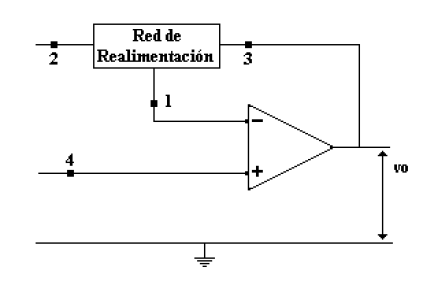
\includegraphics[width=0.45\linewidth,height=0.32\textheight,keepaspectratio]{Imagenes/esquema_realimentado.png}
    \caption{Esquema con red de realimentación}
    \label{fig:esquema_realimentado}
\end{figure}
La estructura básica de utilización de un amplificador operacional incluye una red de realimentación como se observa en la \autoref{fig:esquema_realimentado}. Dependiendo de la terminal donde se aplique la señal se tendrán distintas configuraciones. Las distintas configuraciones dependen de la red de realimentación, siendo las más comúnes: la  \textbf{no inversora} (si se excita en la terminal 4), la \textbf{inversora} (si se excita en la terminal 2) y la \textbf{diferencial}(si
se excita en las terminales 2 y 4).

\subsubsection{Configuración no inversora}
 \begin{figure}[H]
    \centering
    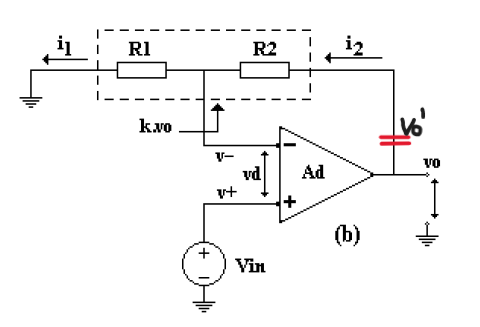
\includegraphics[width=0.5\linewidth,height=0.32\textheight,keepaspectratio]{Imagenes/config_no_inv.png}
    \caption{VFA en configuración no inversora}
    \label{fig:config_no_inv.png}
\end{figure}

Partiendo del circuito de la \autoref{fig:config_no_inv.png} se calcula la ganancia del mismo en base a la fórmula de Black, la \autoref{eq:ganancia_LC_NI}.

\begin{equation}
    A_{vf(NI)} = \frac{V_{out}}{V_{in}} = \dfrac{A_{v(NI)}}{1 - T} 
    \label{eq:ganancia_LC_NI}
\end{equation}

Donde se tiene la ganancia de lazo abierto no inversora ($A_{v(NI)}$), la ganancia de lazo ($T$) y el factor de realimentación ($K$):

\begin{align}
    A_{v(NI)} &= \left.\frac{V_o}{V_{in}}\right|_{V_o'=0} = Ad
    \label{eq:gain_LA_NI}\\
    T &= \left.\frac{V_o}{V_{o}'}\right|_{V_{in}=0} = -(\dfrac{R1}{R1+R2})\cdot Ad = - K \cdot A_{v(NI)}
    \label{eq:gain_lazo_NI}\\
    K &= (\dfrac{R1}{R1+R2})
    \label{eq:K_NI}
\end{align}

Considerando un comportamiento ideal ($ A_{d}(s) \xrightarrow[]{}{\infty}$) y reemplazando los valores de la \autoref{eq:gain_LA_NI} y la \autoref{eq:gain_lazo_NI} en la \autoref{eq:ganancia_LC_NI}  se obtiene el valor de la ganancia a lazo cerrado descripta en la \autoref{eq:ganancia_LC_NI_2}.

\begin{equation}
    A_{v(LC)} = \frac{V_{out}}{V_{in}} = \dfrac{R_2 + R_1}{R_1} = 1 + \dfrac{R2}{R1} 
    \label{eq:ganancia_LC_NI_2}
\end{equation}

\subsubsection{Errores en corriente contínua:}
 Los amplificadores operacionales tienen errores estáticos (o en corriente contínua) y dinámicos (en corriente alterna) que lo alejan de su comportamiento ideal.

 Como el objetivo del presente trabajo consiste en el comportamiento de las respuesta en frecuencia se mencionan los errores estáticos de forma anecdótica:
\begin{itemize}
    \item Off-set de tensión de entrada ($V_{OS}$).
    \item Off-set de corriente de entrada ($I_{OS}$).
    \item Error debido a la ganancia diferencial de lazo abierto finita ($A_d \neq \infty $).
    \item Error debido a la ganancia común de lazo abierto no nula ($A_c \neq 0$).
\end{itemize}
 
\subsubsection{Respuesta en Frecuencia}
Los errores dinámicos se asocian a la disminución de la ganancia a lazo abierto $A_{d(LA)}(s)$ en función de la frecuencia, debido a los polos internos del amplificador operacional.
Partiendo de un modelo básico de un amplificador con un solo polo y una ganancia diferencial definida por la \autoref{eq:gain_LA_rta_frec}

\begin{equation}
    A_d(s) = \frac{A_d(0)}{1 + \frac{s}{\omega_1}}
    \label{eq:gain_LA_rta_frec}
\end{equation}

Aplicando la fórmula de Black para el cálculo de la ganancia a lazo cerrado de este amplificador en \textbf{configuración no inversora} se obtiene la \autoref{eq:gain_LC_rta_frec}.

\begin{equation}
    A_{vf}(s) = \left[\frac{A_d(0)}{1+K.A_d(0)}\right]\cdot\left[\frac{1}{1+\dfrac{s}{\omega_1\cdot(1+K.A_d(0))}}\right] = \frac{A_{vf}(0)}{\left(1+\dfrac{s}{\omega_H}\right)}
    \label{eq:gain_LC_rta_frec}
\end{equation}


Se observa que al aplicar realimentación negativa mediante un factor $K$, el polo del sistema se desplaza hacia altas frecuencias, expandiendo el ancho de banda a lazo cerrado ($\omega_H$). Dicho ancho de banda está dado por la \autoref{eq:frecuencia_high}.

\begin{equation}
    \omega_H = \omega_1 \cdot (1- T_o) = \omega_1 \cdot (1+ K \cdot A_d(0)) \cong \omega_1 \cdot K \cdot A_d(0)) = \omega_T \cdot K
    \label{eq:frecuencia_high}
\end{equation}
Tal que el \textbf{producto de la ganancia (GBW) por el ancho de banda se mantiene constante}, como se observa en la \autoref{eq:GBW_cte}.

\begin{equation}
    GBW = A_{vf}(0) \cdot \omega_H = A_d(0) \cdot \omega_1 = \omega_T = cte
    \label{eq:GBW_cte}
\end{equation}

\begin{figure}[H]
    \centering
    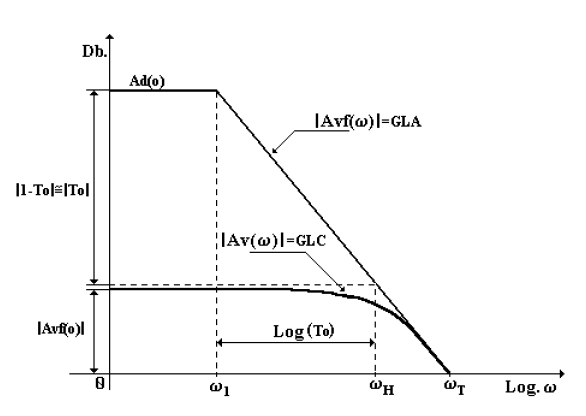
\includegraphics[width=0.5\linewidth,height=0.32\textheight,keepaspectratio]{Imagenes/ganancia_db_marco_teorico.png}
    \caption{Respuesta en frecuencia de un VFA a lazo abierto vs a lazo cerrado}
    \label{fig:ganancia_db_marco_teorico}
\end{figure}

En la \autoref{fig:ganancia_db_marco_teorico} se observa como al introducir una realimentación se aumenta el ancho de banda a costa de una reducción considerable de la ganancia del sistema. Se observa que $\omega_T$ corresponde a la frecuencia para la cual el módulo de la ganancia en decibeles es nula, es decir, ganancia unitaria (en veces).

\subsection{Amplificadores Realimentados por Corriente (CFA)}
El Amplificador Realimentado por Corriente (CFA), o amplificador de transimpedancia, posee una arquitectura interna diferente, requiriendo un menor número de etapas, lo que se traduce en velocidades de operación drásticamente superiores (mayores a $100\text{ MHz}$) y Slew-Rates que pueden superar los $1000\text{ V/}\mu\text{s}$.

\subsubsection{Características Principales}

\begin{figure}[H]
    \centering
    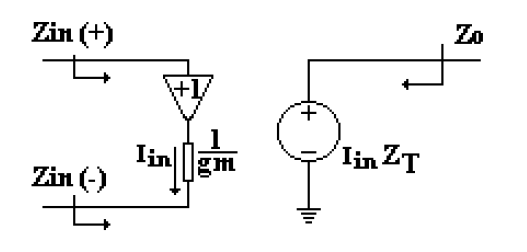
\includegraphics[width=0.5\linewidth,height=0.32\textheight,keepaspectratio]{Imagenes/modelo_CFA.png}
    \caption{Modelo compacto del CFA}
    \label{fig:modelo_CFA}
\end{figure}

A diferencia del VFA, el CFA presenta una arquitectura asimétrica en sus terminales de entrada. El terminal no inversor posee una alta impedancia (entrada a un buffer), mientras que el terminal inversor presenta una impedancia muy baja (típicamente alrededor de $20\,\Omega$, siendo la salida de dicho buffer).

En el CFA, la tensión del terminal de salida es proporcional a la corriente de error que ingresa por el terminal inversor ($I_{in}$). Por ende, el parámetro de transferencia es una transimpedancia ($Z_t$), $V_o = Z_t\,I_{in}$. En la banda de utilización puede modelarse con un único polo, pero para estudiar la estabilidad y las frecuencias altas se requiere el modelo de dos polos del apunte, \autoref{eq:trasimpedancia}:

\begin{equation}
    Z_t(s) = \frac{R_t}{\left(1 + \dfrac{s}{\omega_{t1}}\right)\left(1 + \dfrac{s}{\omega_{t2}}\right)} \qquad \omega_{t1} = \frac{1}{R_t\,C_t}
    \label{eq:trasimpedancia}
\end{equation}

Donde $R_t$ es la transresistencia (del orden del megaohm; \SI{2,37}{M\ohm} para el LM6181), $C_t$ es la transcapacitancia interna (del orden de pocos picofaradios; \SI{4,8}{pF} para el LM6181, \autoref{tab:param_cfa}), $f_{t1}=\SI{14}{kHz}$ es el polo dominante y $f_{t2}=\SI{82,3}{MHz}$ es el segundo polo, de alta frecuencia. La consigna provee $R_t$ y el apunte los polos; por eso se trabaja con $Z_t$ de dos polos y no con el modelo simple de un polo.

\subsubsection{Configuración no inversora}
\begin{figure}[H]
    \centering
    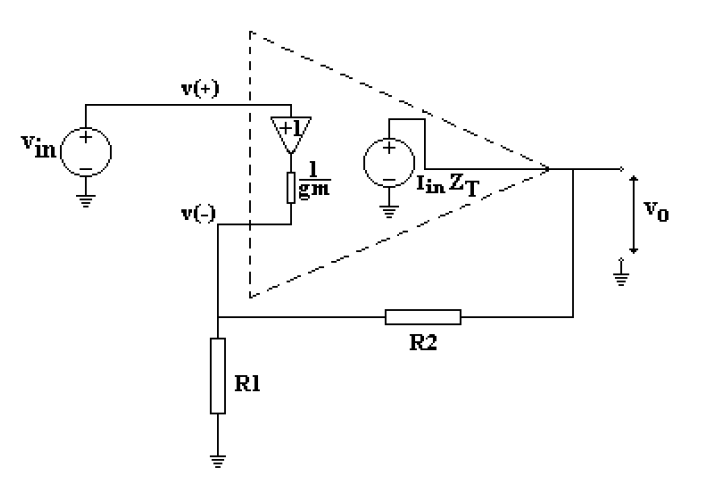
\includegraphics[width=0.5\linewidth,height=0.32\textheight,keepaspectratio]{Imagenes/CFA_NI.png}
    \caption{CFA en configuración no inversora}
    \label{fig:CFA_NI}
\end{figure}

El buffer interno entrega la tensión $V_+$ al terminal inversor a través de su resistencia de salida $r_i$ (baja, del orden de $20$ a $30\,\Omega$; el fabricante no la publica). Sea $I_{in}$ la corriente que entrega el buffer. En el nodo inversor, con $V_n = V_+ - r_i I_{in}$:
\begin{equation}
    I_{in} = \frac{V_n}{R_1} + \frac{V_n - V_o}{R_2} \qquad V_o = Z_t\,I_{in}
\end{equation}
Despejando $I_{in}$ y multiplicando por $R_2$ se obtiene
\begin{equation}
    I_{in}\left[R_2 + r_i\left(1+\tfrac{R_2}{R_1}\right) + Z_t\right] = V_+\left(1+\tfrac{R_2}{R_1}\right)
\end{equation}
Llamando $A_{vfi} = 1 + R_2/R_1$ (ganancia ideal, $Z_t\to\infty$) y $R_{eff} = R_2 + r_i\,A_{vfi}$, la ganancia a lazo cerrado queda
\begin{equation}
    A_{vf}(s) = \frac{A_{vfi}}{1 + \dfrac{R_{eff}}{Z_t(s)}} = \frac{A_{vfi}\,Z_t}{Z_t + R_{eff}}
    \label{eq:Avf_CFA_ri}
\end{equation}
que coincide con la expresión del apunte (Ec.~3.12). La ganancia de lazo es $T(s) = -Z_t(s)/R_{eff}$: depende de $Z_t$ y de $R_{eff}$, \emph{no} de la ganancia $A_{vfi}$ más que a través del término $r_i A_{vfi}$.

\subsubsection{Respuesta en Frecuencia y Estabilidad}
La principal ventaja de la arquitectura CFA reside en su respuesta dinámica. Con $Z_t$ de un polo, $Z_t \cong R_t/(1+sR_tC_t)$, y $R_t \gg R_{eff}$, la \autoref{eq:Avf_CFA_ri} resulta
\begin{equation}
    A_{vf}(s) \cong \frac{A_{vfi}}{1 + s\,C_t\,R_{eff}} \qquad \omega_H \cong \frac{1}{C_t\,R_{eff}} \cong \frac{1}{C_t\,R_2}
    \label{eq:wH_CFA}
\end{equation}
donde la última igualdad vale cuando $r_iA_{vfi} \ll R_2$. El ancho de banda queda fijado casi por completo por $R_2$ y $C_t$, y es prácticamente independiente de la ganancia: para cambiar $A_{vfi}$ se varía solo $R_1$. Esto rompe con la limitación $f_T = A_{vf}\cdot BW$ de los VFA. Cuando $A_{vfi}$ es grande, el término $r_iA_{vfi}$ no es despreciable y el ancho de banda decrece, razón por la cual el diseño usa $R_{eff}$.

Debido a que el ancho de banda es fijado por $R_{eff}$, la resistencia $R_2$ no puede elegirse arbitrariamente: se utiliza como herramienta de diseño para asegurar el margen de fase. Con el segundo polo de $Z_t$, la ganancia de lazo se cruza con 0 dB donde $|Z_t| = R_{eff}$, es decir $f_{cruce} \cong f_{t1}\,R_t/R_{eff}$, y el margen de fase es
\begin{equation}
    M_{\varphi,CFA} = 180^\circ - \left|\angle Z_t(jf_{cruce})\right| \cong 90^\circ - \arctan\frac{f_{cruce}}{f_{t2}}
    \label{eq:Mphi_CFA}
\end{equation}
Un $R_{eff}$ pequeño lleva el cruce hacia $f_{t2}$ y degrada el margen de fase; uno grande lo mejora pero reduce el ancho de banda. El fabricante recomienda $R_2 = \SI{820}{\ohm}$ para el LM6181 (el apunte indica valores cercanos a $1\,\mathrm{k}\Omega$) como compromiso entre velocidad y estabilidad.

\subsection{Estabilidad en Amplificadores}

La estabilidad de un amplificador realimentado es un aspecto relevante en el diseño, ya que determina la capacidad del sistema para operar sin oscilaciones indeseadas. El análisis de estabilidad se puede evaluar a través de la función de transferencia a lazo abierto $|A_v(jw)|$ o de la función de ganancia de lazo $|T(jw)|$, observando su comportamiento en el dominio de la frecuencia y su impacto en la respuesta transitoria.

Para ello se utiliza el método gráfico donde si se usa la función de $|A_v(jw)|$ se busca su intersección con la recta de valor $\frac{1}{K}$ o en el caso de usar la función de $|T(jw)|$ se busca su intersección con $|T(jw)|=0\ dB$. Mediante estos puntos se determinan las condiciones de estabilidad: el margen de fase $M_\phi$ y el margen de ganancia $M_G$.

\subsubsection{Margen de Fase y Margen de Ganancia}

Para cuantificar qué tan alejado se encuentra un sistema del punto crítico de inestabilidad, se definen dos métricas fundamentales sobre el diagrama de Bode de la ganancia de lazo abierto $T(j\omega)$:

\begin{itemize}
    \item \textbf{Margen de Fase ($M\phi$):} Se define como el desfasaje adicional que puede introducirse en el lazo, evaluado en la frecuencia de cruce de ganancia $\omega_{gc}$ (donde el módulo $|T(j\omega_{gc})| = 1$ o $0\text{ dB}$), antes de que el sistema alcance el límite teórico de inestabilidad ($-180^\circ$). Matemáticamente se expresa como:
    \begin{equation}
        MF = 180^\circ + \angle T(j\omega_{gc})
    \end{equation}

    \item \textbf{Margen de Ganancia (MG):} Representa el incremento adicional de ganancia que el sistema puede tolerar antes de volverse inestable. Se evalúa en la frecuencia de cruce de fase $\omega_{pc}$, donde el desfasaje de la función de lazo alcanza exactamente los $-180^\circ$. Se calcula en decibelios a través de la expresión:
    \begin{equation}
        MG = -20 \log_{10} |T(j\omega_{pc})|
    \end{equation}
\end{itemize}

\subsubsection{Medición del Margen de Fase a través de la Respuesta al Escalón}
\label{sec:escalon_mf}

Aunque el margen de fase es un concepto puramente del dominio de la frecuencia, existe una correlación analítica directa con el dominio del tiempo para sistemas dominados por una dinámica de segundo orden. Esta relación permite estimar la estabilidad observando la respuesta transitoria frente a una excitación escalón.

Cuando un sistema de segundo orden subamortiguado es excitado, la tensión de salida presenta un sobrepico antes de alcanzar su valor de estado estacionario. El sobrepico porcentual ($\mathrm{\char37}OS$) se calcula midiendo la diferencia entre la tensión pico $V_{pico}$ y la tensión final $V_{estacionario}$:
\begin{equation}
    \mathrm{\char37}OS = \frac{V_{pico} - V_{estacionario}}{V_{estacionario}} \cdot 100
    \label{eq:OS}
\end{equation}

La magnitud de este sobrepico está directamente vinculada al factor de amortiguamiento $\zeta$ del sistema equivalente mediante la siguiente relación analítica:
\begin{equation}
    \zeta = \frac{-\ln\left(\frac{\mathrm{\char37}OS}{100}\right)}{\sqrt{\pi^2 + \ln^2\left(\frac{\mathrm{\char37}OS}{100}\right)}}
    \label{eq:zeta}
\end{equation}

A su vez, el factor de amortiguamiento $\zeta$ define de manera unívoca el margen de fase del circuito cerrado. Para el análisis teórico riguroso, la relación trigonométrica exacta entre ambas variables está dada por:
\begin{equation}
    MF = \arctan\left( \frac{2\zeta}{\sqrt{\sqrt{1+4\zeta^4}-2\zeta^2}} \right)
    \label{eq:MF_exacta}
\end{equation}

De manera práctica, para valores moderados del amortiguamiento ($0{,}5 \lesssim \zeta \lesssim 0{,}6$) se admite una aproximación lineal, con un error menor a $2^\circ$:
\begin{equation}
    MF \approx 100 \cdot \zeta \quad \text{(en grados)}
    \label{eq:MF_aprox}
\end{equation}
Para máxima planicidad de módulo ($\zeta = 0{,}707$) esta aproximación sobreestima el margen de fase en unos $5^\circ$ (resulta $70{,}7^\circ$ frente a $65{,}5^\circ$ exactos), por lo que en este trabajo se utiliza la relación exacta (\autoref{eq:MF_exacta}).

En consecuencia, el registro y medición de la respuesta al escalón (ya sea mediante simulación o instrumentación física) constituye un método robusto para deducir el amortiguamiento $\zeta$ y, consecuentemente, certificar el margen de fase y la estabilidad del amplificador compuesto.

\subsubsection{Respuesta de máxima planicidad de módulo (MPM)}
\label{sec:mpm}

Un sistema realimentado cuya ganancia de lazo $T(s)$ tiene dos polos presenta también una ganancia a lazo cerrado con dos polos, cuyo carácter (reales o complejos conjugados) depende de la cantidad de realimentación introducida. Si el numerador no tiene ceros, la respuesta normalizada respecto de su valor en continua y de la frecuencia de los polos $\omega_p$ (módulo de los polos, o frecuencia natural), con $S = s/\omega_p$ y $\Omega = \omega/\omega_p$, es:
\begin{equation}
    a_f(S) = \frac{A_{vf}(s)}{A_{vf}(0)} = \frac{1}{1 + \dfrac{S}{Q_p} + S^2}
    \label{eq:2orden}
\end{equation}
donde $Q_p$ es el factor de calidad de los polos ($\zeta = 1/2Q_p$). Su módulo al cuadrado resulta:
\begin{equation}
    |a_f(j\Omega)|^2 = \frac{1}{(1-\Omega^2)^2 + \dfrac{\Omega^2}{Q_p^2}} = \frac{1}{1 + \left(\dfrac{1}{Q_p^2}-2\right)\Omega^2 + \Omega^4}
    \label{eq:mod2orden}
\end{equation}

\paragraph{Condición de máxima planicidad.} Para que el módulo sea constante con la frecuencia, los coeficientes de las potencias homólogas del numerador y del denominador de $|a_f|^2$ deben ser iguales. Como el numerador es la unidad (sus coeficientes son nulos), la única condición que puede satisfacerse es anular el coeficiente de $\Omega^2$:
\begin{equation}
    \frac{1}{Q_p^2} - 2 = 0 \quad \Rightarrow \quad Q_p = \frac{1}{\sqrt{2}} = 0{,}707
    \label{eq:Q_MPM}
\end{equation}
En ese caso el módulo queda $|a_f(j\Omega)|^2 = 1/(1+\Omega^4)$ (respuesta de Butterworth), sin sobrepico. La frecuencia de corte a $-3\text{ dB}$ se obtiene de $1/(1+\Omega_H^4) = 1/2$, es decir $\Omega_H = 1$:
\begin{equation}
    \omega_H = \omega_p
    \label{eq:wH_wp}
\end{equation}
Esto es, en MPM el ancho de banda real coincide con la frecuencia natural de los polos. Para un $Q_p$ cualquiera, la frecuencia de corte surge de igualar a $2$ el denominador de \autoref{eq:mod2orden}:
\begin{equation}
    \Omega_H^2 = a + \sqrt{a^2+1}, \quad a = 1 - \frac{1}{2Q_p^2} \qquad\Rightarrow\qquad f_H = f_p\sqrt{a + \sqrt{a^2+1}}
    \label{eq:polos_BW}
\end{equation}
(para $Q_p = 1/\sqrt{3}$, máxima planicidad de retardo, resulta $f_H = 0{,}786\,f_p$). Los polos de lazo cerrado son $s_{1,2} = -\dfrac{\omega_p}{2Q_p} \pm j\,\omega_p\sqrt{1 - \dfrac{1}{4Q_p^2}}$, que para MPM forman un ángulo de $45^\circ$ con el eje real: $s_{1,2} = -\dfrac{\omega_p}{\sqrt{2}}(1 \mp j)$.

\paragraph{Ganancia de lazo asociada.} Con la fórmula de Black modificada $A_{vf}(s) = A_{vfi}/(1 - 1/T(s))$ y la \autoref{eq:2orden}, resulta $1 - 1/T = 1 + S/Q_p + S^2$, y por lo tanto la ganancia de lazo normalizada es:
\begin{equation}
    T(S) = -\frac{1}{\dfrac{S}{Q_p} + S^2} = -\frac{1}{S\left(S + \dfrac{1}{Q_p}\right)}
    \label{eq:T_norm}
\end{equation}
Es decir, un polo en el origen (el polo dominante $\omega_{p1}$, despreciable frente a $\omega_p$) y otro en $\omega_p/Q_p = \sqrt{2}\,\omega_p$.

\paragraph{Punto crítico y margen de fase.} La frecuencia crítica $\Omega_G$ se obtiene imponiendo $|T(j\Omega_G)| = 1$ en la \autoref{eq:T_norm}:
\begin{equation}
    \Omega_G^4 + \frac{1}{Q_p^2}\,\Omega_G^2 - 1 = 0 \;\;\xrightarrow{\;Q_p = 1/\sqrt{2}\;}\;\; \Omega_G = 0{,}644 \quad\Rightarrow\quad \omega_{Gc} = 0{,}644\,\omega_p
    \label{eq:omegaG}
\end{equation}
donde $\omega_{Gc}$ es la frecuencia de cruce de la ganancia de lazo \emph{compensada} (en el apunte de la cátedra se la denomina $\omega_G$; aquí se la distingue del ancho de banda potencial, \autoref{sec:bw}). El margen de fase resulta:
\begin{equation}
    M_\varphi = 180^\circ + \angle T(\Omega_G) = 180^\circ - 90^\circ - \arctan\left(\Omega_G\,Q_p\right) = 65{,}5^\circ
    \label{eq:Mphi_MPM}
\end{equation}
que es el valor especificado en la consigna ($M_\varphi \approx \ang{65}$ o, equivalentemente, $Q_p = 0{,}707$) y coincide con el obtenido de la \autoref{eq:MF_exacta} para $\zeta = 1/(2Q_p) = 0{,}707$.

\paragraph{Relaciones de diseño.} En un amplificador compuesto la ganancia de lazo puede aproximarse con dos polos, $\omega_{p1} \ll \omega_{p2}$:
\begin{equation}
    T(s) = - \frac{T_0}{\left(1 + \dfrac{s}{\omega_{p1}}\right)\left(1 + \dfrac{s}{\omega_{p2}}\right)} \qquad T_0 = |T(0)|
    \label{eq:lazo2polos}
\end{equation}
Introduciendo esta expresión en la fórmula de Black modificada:
\begin{equation}
    A_{vf}(s) = \frac{A_{vfi}}{1 + \dfrac{1}{T_0}\left(1+\dfrac{s}{\omega_{p1}}\right)\left(1+\dfrac{s}{\omega_{p2}}\right)} \cong \frac{A_{vfi}}{1 + \dfrac{s}{T_0\,\omega_{p1}} + \dfrac{s^2}{T_0\,\omega_{p1}\,\omega_{p2}}}
    \label{eq:Avf_dospolos}
\end{equation}
donde se utilizaron $T_0 \gg 1$ y $D_p = \omega_{p2}/\omega_{p1} \gg 1$ (separación de polos). Comparando con la \autoref{eq:2orden}, y definiendo $A = T_0/D_p$:
\begin{equation}
    \omega_p^2 = T_0\,\omega_{p1}\,\omega_{p2} \;\Rightarrow\; \omega_p = \omega_{p2}\sqrt{A} \qquad\qquad \frac{1}{Q_p} = \frac{\omega_p}{T_0\,\omega_{p1}} = \frac{1}{\sqrt{A}} \;\Rightarrow\; Q_p^2 = A = \frac{T_0}{D_p}
    \label{eq:wp_A}
\end{equation}
Para MPM ($Q_p^2 = 1/2$) la separación de polos debe ser, entonces:
\begin{equation}
    D_p = 2\,T_0 \qquad\Rightarrow\qquad \omega_p = \frac{\omega_{p2}}{\sqrt{2}}
    \label{eq:Dp_MPM}
\end{equation}
Por último, el margen de fase de un lazo de dos polos cualquiera se calcula en su frecuencia crítica $f_{Gc}$, solución de $|T(j2\pi f_{Gc})| = 1$:
\begin{equation}
    M_\varphi = 180^\circ - \arctan\frac{f_{Gc}}{f_{p1}} - \arctan\frac{f_{Gc}}{f_{p2}}
    \label{eq:Mphi_2polos}
\end{equation}
Con $\omega_{p1}\to 0$ y $\omega_{p2} = \sqrt{2}\,\omega_p$ esta expresión coincide con la \autoref{eq:Mphi_MPM}.

\subsection{Amplificadores compuestos}

Se entiende por estructuras compuestas a aquellas configuraciones que incorporan más de un amplificador participando dentro del lazo de realimentación principal. El objetivo de esta topología es lograr un comportamiento global que conserve y potencie las características relevantes de cada dispositivo individual, minimizando al mismo tiempo sus debilidades intrínsecas. Una de las conexiones más utilizadas consiste en disponer dos amplificadores operacionales en cascada dentro del lazo, como se observa en la \autoref{fig:MT_AO_compuesto}.

\begin{figure}[H]
    \centering
    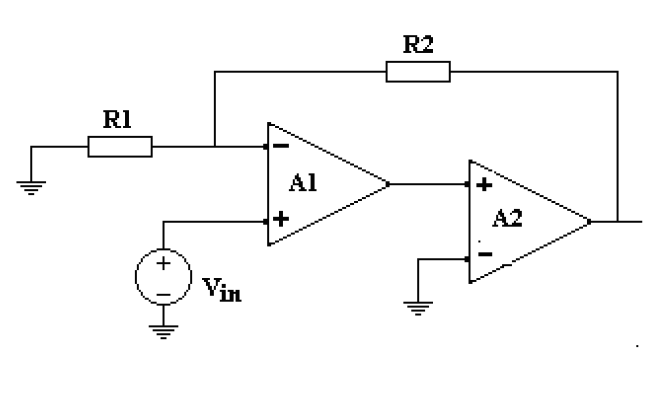
\includegraphics[width=0.5\linewidth,height=0.32\textheight,keepaspectratio]{Imagenes/MT_AO_compuesto.png}
    \caption{Amplificador compuesto}
    \label{fig:MT_AO_compuesto}
\end{figure}

Si bien la topología compuesta mejora considerablemente las características del circuito al usarse con amplificadores con características distintas se plantea el caso teórico de utilizar dos amplificadores idénticos, con el mismo modelo y topología.

\begin{figure}[H]
    \centering
    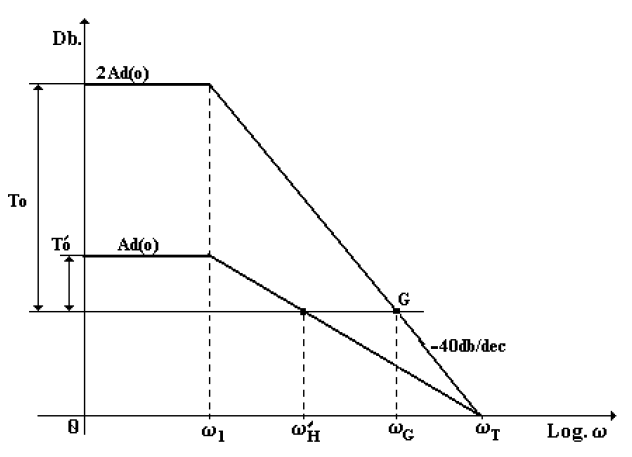
\includegraphics[width=0.5\linewidth,height=0.32\textheight,keepaspectratio]{Imagenes/MT_AO_compuesto_rta_frec.png}
    \caption{Respuesta en frecuencia del amplificador compuesto}
    \label{fig:MT_AO_compuesto_rta_frec}
\end{figure}

Como se observa en la \autoref{fig:MT_AO_compuesto_rta_frec}, la ganancia de lazo abierto del sistema compuesto se incrementa significativamente ($2 \cdot A_{d0}$) y también se introduce un polo doble $\omega_1$. Al compararse con la respuesta en frecuencia de una configuración de un solo amplificador se observa que para una misma ganancia $\frac{1}{K_c}$ el circuito con los amplificadores compuestos obtienen un ancho de banda mucho mayor ($\omega_G > \omega_H$).

Este polo doble puede inducir un desfase excesivo, reduciendo el margen de fase y comprometiendo la estabilidad del sistema. Por lo tanto, es crucial implementar técnicas de compensación para garantizar un comportamiento estable y predecible del amplificador compuesto.


\subsubsection{Ancho de banda potencial y ancho de banda real}
\label{sec:bw}

En el análisis de los amplificadores compuestos se emplean varias frecuencias que conviene distinguir, porque se obtienen de curvas distintas y con criterios distintos:

\begin{itemize}
    \item \textbf{Ancho de banda potencial ($f_G$):} es la frecuencia del punto crítico $G$ de la estructura, donde la ganancia de lazo cruza $0\text{ dB}$ (o, equivalentemente, donde la ganancia de lazo abierto $|A_v|$ se iguala a $1/K$). Representa el máximo ancho de banda que admite la estructura para la ganancia $A_{vf}$ pedida. Se calcula a partir de la ganancia de lazo y no se mide directamente sobre $A_{vf}(s)$.
    \item \textbf{Ancho de banda real ($f_H$):} es la frecuencia a la que el módulo de la ganancia a lazo cerrado cae $3\text{ dB}$ respecto de su valor en continua, $|A_{vf}(j\omega_H)| = A_{vf}(0)/\sqrt{2}$. Se puede calcular a partir de la función de transferencia a lazo cerrado (\autoref{eq:polos_BW}) y se puede medir sobre el circuito simulado o armado.
    \item \textbf{Frecuencia de los polos de lazo cerrado ($f_p$):} es el módulo de los polos de la función de transferencia a lazo cerrado (frecuencia natural, \autoref{eq:wp_A}). Para $Q_p = 1/\sqrt{2}$ coincide con el ancho de banda real (\autoref{eq:wH_wp}).
\end{itemize}

Cuando la respuesta es de máxima planicidad de módulo ($Q_p = 1/\sqrt{2}$) las tres magnitudes anteriores se relacionan de forma simple: el ancho de banda real coincide con la frecuencia de los polos y, para el compuesto compensado por desplazamiento (\autoref{eq:wH_MPM}), también con el ancho de banda potencial:
\begin{equation}
    f_H = f_p = f_G \qquad (Q_p = 1/\sqrt{2})
    \label{eq:fH_fp_MPM}
\end{equation}
Para cualquier otro $Q_p$ la igualdad no se cumple: con $Q_p<1/\sqrt{2}$ la respuesta es más amortiguada y $f_H$ difiere de $f_p$ (\autoref{eq:wH_wp}).

\paragraph{Amplificador simple.} De la \autoref{eq:frecuencia_high}, el ancho de banda del amplificador con una sola etapa es
\begin{equation}
    f_H' \cong K\, f_T = \frac{f_T}{A_{vf}}
    \label{eq:bw_simple}
\end{equation}

\paragraph{Amplificador compuesto sin compensar.} Este resultado es el del apunte (Cap.~VII, Fig.~7.18). Para $\omega \gg \omega_1$ cada amplificador se comporta como $A_d(j\omega) \cong \omega_T/(j\omega)$, de modo que con dos amplificadores idénticos $|A_v(j\omega)| \cong (\omega_T/\omega)^2$. El punto crítico se obtiene de la condición $|A_v(j\omega_G)| = 1/K = A_{vf}$:
\begin{equation}
    \omega_G = \frac{\omega_T}{\sqrt{A_{vf}}} \qquad\Rightarrow\qquad \frac{f_G}{f_H'} = \sqrt{A_{vf}}
    \label{eq:wG}
\end{equation}
Es decir, el ancho de banda potencial del compuesto es función inversa de la raíz cuadrada de la ganancia a lazo cerrado, y mejora en un factor $\sqrt{A_{vf}}$ al del amplificador simple. Sin embargo, el cruce ocurre con una pendiente de $-40\text{ dB/dec}$ (polo doble), por lo que el margen de fase es prácticamente nulo y es necesario compensar.

\paragraph{Amplificador compuesto compensado por desplazamiento.} Al compensar, la ganancia de lazo cruza $0\text{ dB}$ con pendiente de $-20\text{ dB/dec}$. En la zona $\omega_1 \ll \omega \ll \omega_{px}$ resulta $|T| \cong T_0\,\omega_1/\omega = K\,A_{vf2}\,\omega_T/\omega$, de donde
\begin{equation}
    \omega_{Gc} \cong K\, A_{vf2}\,\omega_T
    \label{eq:wGc}
\end{equation}
Esta frecuencia de cruce de la ganancia de lazo \textbf{compensada} ($f_{Gc}$) es la que se mide en el simulador sobre el circuito de ganancia de lazo y con la que se calcula el margen de fase. Es menor que el potencial, porque la compensación reduce la ganancia de lazo. En cambio, el ancho de banda real de la respuesta a lazo cerrado con máxima planicidad vale (\autoref{sec:mpm}) $f_H = f_p = f_{px}/\sqrt{2}$, que con $A_{vf2} = Q_p\sqrt{A_{vf}}$ (\autoref{eq:Avf2_MPM}) resulta
\begin{equation}
    f_H = \frac{f_{px}}{\sqrt{2}} = \frac{f_T}{\sqrt{2}\,A_{vf2}} = \frac{f_T}{\sqrt{A_{vf}}} = f_G
    \label{eq:wH_MPM}
\end{equation}
En consecuencia, la compensación por desplazamiento \textbf{recupera como ancho de banda real el ancho de banda potencial} del compuesto sin compensar, a costa de perder ganancia de lazo (precisión estática). Además, para MPM se verifica $f_H = \sqrt{2}\,f_{Gc}$.

\begin{table}[H]
\centering
\caption{Resumen de las frecuencias características del amplificador compuesto.}
\label{tab:resumen_bw}
\small
\begin{tabularx}{\textwidth}{>{\raggedright\arraybackslash}p{3.6cm} >{\raggedright\arraybackslash}X >{\raggedright\arraybackslash}X}
\toprule
\textbf{Magnitud} & \textbf{Definición} & \textbf{Cómo se obtiene} \\
\midrule
Ancho de banda potencial $f_G$ & Punto crítico $G$ de la estructura sin compensar ($|T| = 1$ con $-40\text{ dB/dec}$) & Cálculo: $f_T/\sqrt{A_{vf}}$ \\
Cruce de la ganancia de lazo compensada $f_{Gc}$ & $|T(jf_{Gc})| = 1$ con la compensación implementada & Cálculo: $K\,A_{vf2}\,f_T$. Simulación del circuito de ganancia de lazo \\
Polos de lazo cerrado $f_p$ & Módulo de las raíces de $1 - T(s) = 0$ & Cálculo con \autoref{eq:wp_A} \\
Ancho de banda real $f_H$ & $|A_{vf}(jf_H)| = A_{vf}(0)/\sqrt{2}$ ($-3\text{ dB}$) & Cálculo: \autoref{eq:wH_wp} y \autoref{eq:polos_BW}. Simulación AC o medición \\
\bottomrule
\end{tabularx}
\end{table}

\subsubsection{Compensación por desplazamiento (Separación de polos)}

\begin{figure}[H]
    \centering
    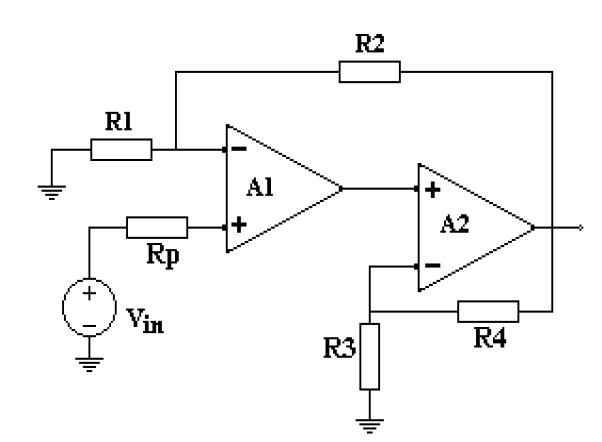
\includegraphics[width=0.5\linewidth,height=0.32\textheight,keepaspectratio]{Imagenes/MT_AO_desplazamiento.png}
    \caption{Esquemático de compensación por desplazamiento de polos}
    \label{fig:MT_AO_desplazamiento}
\end{figure}

Una solución para mitigar la inestabilidad causada por la presencia de un polo doble en la configuración compuesta consiste en separar dichos polos en el dominio de la frecuencia. Esto se logra incrementando la frecuencia de corte (y por ende, el ancho de banda) del segundo amplificador de la cascada.

\begin{figure}[H]
    \centering
    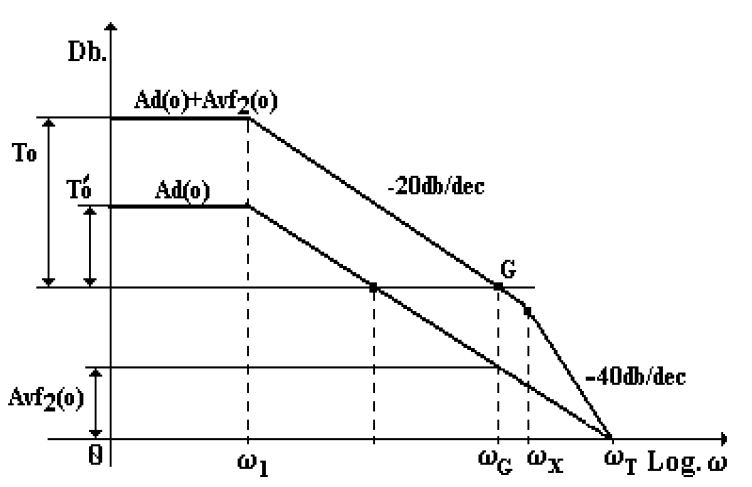
\includegraphics[width=0.5\linewidth,height=0.32\textheight,keepaspectratio]{Imagenes/MT_rta_frec_desplazamiento.png}
    \caption{Respuesta en frecuencia de la compensación por desplazamiento}
    \label{fig:MT_AO_desplazamiento_rta_frec}
\end{figure}

Para lograr este desplazamiento, se reduce la ganancia del segundo amplificador mediante un lazo de realimentación negativa interno o local, como se muestra en la \autoref{fig:MT_AO_desplazamiento}. Al disminuir su ganancia local a un valor $A_{vf2}$, su frecuencia de polo se desplaza hacia altas frecuencias ($\omega_{px}$), permitiendo que la ganancia de lazo global del sistema compuesto ($T$) cruce el eje de 0 dB con una pendiente estable de $-20$ dB/dec antes de que el segundo polo actúe, tal y como se observa en la \autoref{fig:MT_AO_desplazamiento_rta_frec}.


La separación requerida entre el primer polo dominante ($\omega_1$) y el polo desplazado ($\omega_{px}$) dependerá del tipo de respuesta deseada (por ejemplo, Máxima Planicidad de Módulo o MPM). La frecuencia del nuevo polo de compensación del segundo amplificador se determina como:
\begin{equation}
\omega_{px} = \frac{\omega_T}{A_{vf2}(0)}
\label{eq:wpx}
\end{equation}
Donde $\omega_T$ es la frecuencia de transición del amplificador. Si bien esta técnica recupera el ancho de banda potencial estableciendo un margen de fase seguro, se realiza a expensas de sacrificar una fracción de la ganancia de lazo total (precisión estática), ya que se reduce la ganancia de la segunda etapa.

\paragraph{Origen de $\omega_{px}$.} Con el lazo local de factor $K_2 = 1/A_{vf2}$ y un amplificador de un polo dominante, $A_2(s) = A_{d0}/(1+s/\omega_1)$, la ganancia de la segunda etapa realimentada es
\begin{equation}
    A_{2f}(s) = \frac{A_2}{1+K_2 A_2} = \frac{A_{d0}}{1 + \dfrac{A_{d0}}{A_{vf2}} + \dfrac{s}{\omega_1}} \cong \frac{A_{vf2}}{1 + \dfrac{s}{\omega_{px}}} \qquad \omega_{px} = \omega_1\left(1 + \frac{A_{d0}}{A_{vf2}}\right) \cong \frac{\omega_T}{A_{vf2}}
    \label{eq:A2f}
\end{equation}
es decir que el producto ganancia-ancho de banda se mantiene constante y el polo se desplaza hacia altas frecuencias al reducir la ganancia.

\paragraph{Condición de diseño para MPM.} La ganancia de lazo del compuesto queda con dos polos, $\omega_1$ y $\omega_{px}$ (\autoref{eq:lazo2polos} con $\omega_{p1} = \omega_1$ y $\omega_{p2} = \omega_{px}$), con
\begin{equation}
    T_0 = K\,A_{d0}\,A_{vf2} \qquad D_p = \frac{\omega_{px}}{\omega_1} = \frac{A_{d0}}{A_{vf2}}
\end{equation}
Reemplazando en la \autoref{eq:wp_A} se tiene $Q_p^2 = T_0/D_p = K\,A_{vf2}^2$, y al imponer $Q_p = 1/\sqrt{2}$ (equivalentemente $D_p = 2T_0$, \autoref{eq:Dp_MPM}) resulta la ganancia que debe tener la segunda etapa:
\begin{equation}
    A_{vf2} = \frac{Q_p}{\sqrt{K}} = Q_p\sqrt{A_{vf}}
    \label{eq:Avf2_MPM}
\end{equation}
\paragraph{Verificación sin aproximar.} Sin suponer $T_0 \gg 1$ ni $D_p \gg 1$, los polos de $1 - T(s) = 0$ cumplen $s^2 + (\omega_1 + \omega_{px})\,s + \omega_1\omega_{px}(1+T_0) = 0$, de donde $\omega_p^2 = \omega_1\omega_{px}(1+T_0)$ y $Q_p = \omega_p/(\omega_1+\omega_{px})$. Para el LM324, $Q_p^2$ exacto difiere de $1/2$ en un orden de $10^{-5}$, por lo que las aproximaciones de la \autoref{eq:wp_A} son válidas. Este cálculo exacto es el que realiza el cuaderno.


\subsubsection{Amplificadores compuestos de distinta topología (VFA + CFA)}
\label{sec:compuesto_distinto}

El apunte desarrolla el amplificador compuesto con dos amplificadores idénticos; no trata el caso de un VFA seguido de un CFA. Este caso es el que utiliza la técnica de ``composite amplifier'' de la literatura de aplicación (Loquinario, \emph{Analog Dialogue} 53-03, 2019): un VFA de precisión y baja tensión de offset, pero lento, se combina con un amplificador rápido dentro del mismo lazo, de modo que la exactitud en continua la fija el primero y el ancho de banda el segundo. El tratamiento que sigue es una extensión directa de las relaciones del apunte.

Sea el VFA (A01) con ganancia $A_1(s)$ y el CFA (A02) con su realimentación local. Se llama $A_{vfi2}$ a la ganancia ideal del CFA realimentado (la $A_{vfi}$ de la \autoref{eq:Avf_CFA_ri}, renombrada para distinguirla de la ganancia global) y $A_{2f}(s)$ a su respuesta en frecuencia. Con $K = 1/A_{vf}$ el factor de realimentación global, resulta
\begin{equation}
    A_1(s) = \frac{A_{d0}}{\left(1+\dfrac{s}{\omega_1}\right)\left(1+\dfrac{s}{\omega_2}\right)}
\end{equation}
y la ganancia de lazo global
\begin{equation}
    T(s) = -K\,A_1(s)\,A_{2f}(s)
\end{equation}
Como el polo de $A_{2f}$ es mucho más alto que la frecuencia crítica, en la zona de interés $A_{2f}\cong A_{vfi2}$ y $T$ queda con los dos polos del VFA:
\begin{equation}
    T(s) \cong \frac{T_0}{\left(1+\dfrac{s}{\omega_1}\right)\left(1+\dfrac{s}{\omega_2}\right)} \qquad T_0 = K\,A_{d0}\,A_{vfi2}
\end{equation}
Para $\omega \gg \omega_1$ el VFA se comporta como $\omega_T/s$, y la ganancia de lazo se reduce a $T \cong K\,A_{vfi2}\,\omega_T/s$. Su cruce asintótico ($|T|=1$) define el ancho de banda potencial
\begin{equation}
    \omega_g = K\,A_{vfi2}\,\omega_T \qquad\Rightarrow\qquad A_{vfi2} = \frac{\omega_g}{K\,\omega_T}
    \label{eq:wg_VFACFA}
\end{equation}
A diferencia del compuesto de amplificadores idénticos (donde $f_G = f_T/\sqrt{A_{vf}}$), aquí el ancho de banda lo fija la ganancia del CFA, $A_{vfi2}$. Aplicando la \autoref{eq:wp_A} con $D_p = \omega_2/\omega_1$ resulta
\begin{equation}
    Q_p^2 \cong \frac{T_0}{D_p} = \frac{K\,A_{d0}\,A_{vfi2}\,\omega_1}{\omega_2} = \frac{\omega_g}{\omega_2}
    \label{eq:Qp_VFACFA}
\end{equation}
Para MPM se exige $Q_p^2 = 1/2$, lo que limita el cruce a $\omega_g \le \omega_2/2$ y, por lo tanto, la ganancia del CFA queda acotada:
\begin{equation}
    A_{vfi2} \le A_{vfi2,max} = \frac{\omega_2}{2\,K\,\omega_T}
    \label{eq:Avfi2_max}
\end{equation}
Elegir $A_{vfi2} = A_{vfi2,max}$ da MPM en el modelo de dos polos, pero deja poco margen para los polos del CFA, que agregan atraso de fase. Por eso conviene tomar un $A_{vfi2}$ algo menor, que da $Q_p<1/\sqrt2$ (respuesta más amortiguada, sin pico) y un margen de fase mayor.

Para que la aproximación $A_{2f}\cong A_{vfi2}$ sea válida, el polo del CFA realimentado debe quedar una década por encima de $f_g$. Con $R_{eff}$ definida en la \autoref{eq:Avf_CFA_ri}:
\begin{equation}
    R_{eff} = R_2 + r_i\,A_{vfi2} \qquad f_{cfa} \cong \frac{1}{2\pi\,C_t\,R_{eff}} \ge 10\,f_g
\end{equation}
El modelo completo (cuatro polos) incluye $A_{2f}(s)$ de la \autoref{eq:Avf_CFA_ri}.

\subsubsection{Compensación cero-polo (Adelanto)}
\label{sec:adelanto}
Para aplicaciones de alta ganancia donde se requiere mantener la máxima precisión posible en continua y a su vez estabilizar el sistema frente a polos parásitos o múltiples (como en los amplificadores compuestos), la compensación por adelanto de fase, también conocida como compensación cero-polo, resulta sumamente efectiva.

Esta técnica introduce un cero ($f_{zx}$) cercano al segundo polo problemático del sistema original, de modo que corrige el atraso de fase que éste provoca antes de llegar a la frecuencia del punto crítico. Se implementa con una red resistiva-capacitiva, cuya forma básica es un divisor resistivo $R_x$--$R_y$ con un capacitor $C_x$ en paralelo con $R_x$ (\autoref{fig:red_RC_adelanto}):
\begin{equation}
    \begin{gathered}
    A_c(s) = \frac{R_y}{R_x+R_y}\cdot\frac{1+sC_xR_x}{1+sC_x\,(R_x\parallel R_y)} \\
    \omega_{zx} = \frac{1}{C_xR_x} \qquad \omega_{px} = \frac{1}{C_x\,(R_x\parallel R_y)} \qquad \frac{\omega_{px}}{\omega_{zx}} = 1+\frac{R_x}{R_y}
    \end{gathered}
    \label{eq:red_RC}
\end{equation}
La red atenúa en continua ($A_c(0) = R_y/(R_x+R_y)<1$) y a alta frecuencia recupera la ganancia unitaria; por eso el cero se ubica antes que el polo.

\begin{figure}[H]
    \centering
    \begin{tikzpicture}[x=1cm,y=1cm,line cap=round]
        \draw (0,1.2) node[left]{$v_i$} -- (0.5,1.2);
        \draw (0.5,1.2) -- (0.5,1.8) -- (1.0,1.8); \draw (2.2,1.8) -- (2.7,1.8) -- (2.7,1.2);
        \draw (1.0,1.65) rectangle (2.2,1.95); \node at (1.6,2.25){$R_x$};
        \draw (0.5,1.2) -- (0.5,0.6) -- (1.0,0.6); \draw (1.0,0.45) -- (1.0,0.75); \draw (1.25,0.45) -- (1.25,0.75); \draw (1.25,0.6) -- (2.7,0.6) -- (2.7,1.2);
        \node at (1.1,0.15){$C_x$};
        \draw (2.7,1.2) -- (3.4,1.2) node[right]{$v_o$};
        \draw (3.0,1.2) -- (3.0,0.9); \draw (2.85,0.9) rectangle (3.15,0.3); \node at (3.5,0.6){$R_y$};
        \draw (3.0,0.3) -- (3.0,0.0); \draw (2.8,0.0) -- (3.2,0.0);
    \end{tikzpicture}
    \caption{Red cero-polo: $C_x$ en paralelo con $R_x$ y $R_y$ a tierra}
    \label{fig:red_RC_adelanto}
\end{figure}

Según el lugar del lazo donde se coloca la red, el efecto es diferente (apunte, Cap. VI):
\begin{itemize}
    \item \textbf{Red en la entrada del amplificador compuesto o dentro de la red de realimentación} (por ejemplo, $C_x$ en paralelo con la resistencia de realimentación global): el cero aparece en el numerador de la ganancia de lazo,
    \begin{equation}
        T(s) \cong - \frac{T_0 \left(1 + \frac{s}{\omega_{zx}}\right)}{\left(1 + \frac{s}{\omega_{p1}}\right) \left(1 + \frac{s}{\omega_{p2}}\right)}
    \end{equation}
    y, definiendo $D_z = \omega_{zx}/\omega_{p2}$, la relación $1/Q_p = 1/\sqrt{A} + \sqrt{A}/D_z$ con $A = T_0/D_p$ (apunte, Ec.~6.40a) permite ubicar el cero para MPM. Para $D_p \gg 1$ resulta
    \begin{equation}
        f_{zx} \cong f_{p2}\,Q_p\sqrt{\frac{T_0}{D_p}}
    \end{equation}
    \item \textbf{Red a la salida del amplificador básico} (entre la salida del VFA y la entrada del siguiente amplificador): el cero queda en el numerador de la ganancia a lazo cerrado y se elige $D_x = \omega_{zx}/\omega_{p2} \cong 1$ (apunte, Ec.~6.50 y 6.51), de modo que el cero \emph{cancela} el segundo polo del amplificador. La ganancia de lazo queda con dos polos, $\omega_{p1}$ y el polo de la red $\omega_{px}$, y es éste (más alto que $\omega_{p2}$) el que define el nuevo segundo polo.
\end{itemize}

La ventaja fundamental de la compensación por adelanto es que recupera o extiende el ancho de banda potencial sin degradar la ganancia de lazo en continua $T_0$, siempre que la atenuación $A_c(0)$ de la red se compense con ganancia adicional en alguna etapa (en el compuesto VFA + CFA, retocando $A_{vfi2}$). En la práctica la cancelación es aproximada, pues depende de las tolerancias de $R_x$ y $C_x$ y de la impedancia de salida del amplificador que alimenta a la red. En las expresiones, $Q_p$ y $D_p$ son el factor de calidad y la separación de polos definidos en la \autoref{sec:mpm}.
